\documentclass[11pt]{article}
\usepackage[a4paper,margin=21mm]{geometry}
\usepackage[no-math]{fontspec}
\setmainfont{Latin Modern Roman}
\newfontfamily\CJKfont{Noto Serif CJK SC}
\XeTeXlinebreaklocale "zh"
\XeTeXlinebreakskip=0pt plus 1pt
\usepackage{amsmath,amssymb,amsthm,amscd,graphicx,color}
\usepackage{xurl}
\usepackage[unicode,hidelinks]{hyperref}
\allowdisplaybreaks
\setlength\emergencystretch{3em}
\numberwithin{equation}{section}

\numberwithin{equation}{section}

\newtheorem{Theorem}{Theorem}[section]
\newtheorem{Lemma}[Theorem]{Lemma}

\usepackage{mathtools}
\usepackage[braket, qm]{qcircuit}

\DeclarePairedDelimiter\ceil{\lceil}{\rceil}
\DeclarePairedDelimiter\floor{\lfloor}{\rfloor}

\newcommand{\ea}[1]{\begin{align}#1\end{align}}
\newcommand{\eg}[1]{\begin{gather}#1\end{gather}}
\newcommand{\eat}[2]{\begin{alignat}{#1} #2\end{alignat}}
\newcommand{\nn}{\nonumber \\}
\newcommand{\la}{\langle}
\newcommand{\ra}{\rangle}
\newcommand{\mmod}{\mathrm{~mod~}}
\newcommand{\mcl}{\mathcal}
\newcommand{\mbf}{\mathbf}
\newcommand{\mbb}{\mathbb}
\newcommand{\mrm}{\mathrm}
\newcommand{\bmp}{\begin{pmatrix}}
\newcommand{\emp}{\end{pmatrix}}
\newcommand{\bmb}{\begin{bmatrix}}
\newcommand{\emb}{\end{bmatrix}}
\newcommand{\vpu}[1]{^{\vphantom{#1}}}

\DeclareMathOperator{\tr}{Tr}
\DeclareMathOperator{\ebr}{ebr}
\DeclareMathOperator{\len}{len}
\DeclareMathOperator{\ch}{\mcl{C}}
\DeclareMathOperator{\rank}{Rank}
\DeclareMathOperator{\GL}{GL}
\DeclareMathOperator{\Gal}{Gal}
\DeclareMathOperator{\rel}{Re}
\DeclareMathOperator{\sgn}{Sign}

\begin{document}
\begin{center}\Large Classification of finite-dimensional irreducible projective unitary representations of the triangle group (3,3,3) with primitive commutator parameter\end{center}
\noindent\textbf{Stable ID:} 985\quad\textbf{Author:} Danylo Yakymenko\par
\noindent\textbf{Work:} SICs and the Triangle Group $(3,3,3)$\par
\noindent\textbf{Source:} \url{https://sigma-journal.com/2024/044/}\par
\noindent\textbf{Version:} Official SIGMA 20 (2024) article 044, DOI 10.3842/SIGMA.2024.044; journal PDF and native TeX acquired 2026-09-30, exact bytes pinned by SHA256\par
\noindent\textbf{Rights:} CC BY 4.0. Authors retain copyright. \url{https://creativecommons.org/licenses/by/4.0/}. Reuse and typesetting adaptation; original language and mathematical content preserved.\par
\noindent\textbf{Difficulty (prior selection preserved):} {\CJKfont H2: The author lifts the known finite Weyl-pair representations to the triangle generators and analyzes their cyclic permutation orbit. Generic three-component representations and the exceptional splitting into nine d-dimensional representations require an explicit invariant-subspace construction and an equivalence classification. This classification is counted as one unit, including its exceptional cases.}\par
\medskip\noindent\textbf{Editorial boundary note (not author text):} Complete original Theorem3.1 with the exact primitive commutator, phase/product, unitary-equivalence, generic3d and all nine exceptional d-dimensional cases. The proof is the full preceding author derivation rather than a separately labelled proof: complete Weyl/Clifford/Zauner background and explicit operators, triangle-group projective relations, cyclic orbit and generic block construction, every singular-case invariant subspace, operator action, dimension/irreducibility and equivalence argument are retained. The cited finite Weyl-pair classification is an explicit formal standard prerequisite; the new lift/splitting construction is fully human-authored. The original planar-motion illustration is retained unchanged, with its abstract group presentation, generator rotations and translation directions fully editable in the native text. Real installed qcircuit supplies the original ket/bra notation, without a semantic shim. Later canonical-unitary/SIC applications and the open SIC-conjecture discussion are excluded and not counted. Literal phases, roots, labels and exceptional alternatives remain unchanged; no new proof, mathematical refereeing or notation repair.\par
\medskip\hrule\medskip\noindent\textbf{Author text begins below.}\par
\setcounter{section}{1}
% Original source lines 176--681
\section{Weyl--Heisenberg group and its symmetries}\label{sec:wh}

In this section, we mainly follow Appleby \cite{Appleby}.
Recall that the Weyl--Heisenberg group is generated by
the clock and shift matrices $Z$, $X$:
\[
Z = \bmp
1 & 0 & 0 & \cdots & 0\\
0 & \omega & 0 & \cdots & 0\\
0 & 0 & \omega^2 & \cdots & 0\\
\vdots & \vdots & \vdots & \ddots & \vdots\\
0 & 0 & 0 & \cdots & \omega^{d-1}
\emp,
\qquad
X = \bmp
0 & 0 & \cdots & 0 & 1\\
1 & 0 & \cdots & 0 & 0\\
0 & 1 & \cdots & 0 & 0\\
\vdots & \vdots & \ddots &\vdots &\vdots\\
0 & 0 & \cdots & 1 & 0\\
\emp,
\]
where $\omega = \exp \bigl(\frac{2\pi{\rm i}}{d}\bigr)$.
They satisfy $Z^d = X^d = I$ and a kind of commutation relation $ZX = \omega XZ$.
It is easy to see that each element of the generated group has the
form $\omega^mX^kZ^l$, where $k,l,m \in \mbb{Z}_d$.
For further constructions, it is convenient to also add the factor $\tau = -\exp \bigl(\frac{\pi {\rm i}}{d}\bigr)$ to~it.
We thus define the group by ${\rm WH}(d) = \la X, Z, \tau I \ra$.
Note that $\tau^2 = \omega$ and if $d$ is odd then \smash{$\tau = \omega^{\frac{d+1}{2}}$}
so it adds nothing, but doubles the group in even dimensions.
In any case, for the quotient over the group center, denoted by $\la \xi I \ra$, we have ${\rm WH}(d) / \la \xi I \ra \simeq \mbb{Z}_d \times \mbb{Z}_d$.

The $d^2$ \textit{displacement matrices} for ${\bf a} = (a_1,a_2) \in \mbb{Z}_d^2$ defined by
\[
D_{\bf a} = \tau^{a_1a_2} X^{a_1}Z^{a_2} \in {\rm WH}(d)
\]
are cosets representatives of the quotient group ~${{\rm WH}(d) / \la \xi I \ra}$.
They satisfy the relations $D_{\bf a} D_{\bf b} = \tau^{\la \bf a, b\ra} D_{\bf a+b}$,
where $\la {\bf a, b} \ra = a_2b_1 - b_2a_1$ is the symplectic form.
In particular, $D_{\bf a}^\dag = D_{-\bf a}$.

The Clifford group ${\rm Cli}(d)$ is defined as the group of unitary automorphisms
of the Weyl--Heisenberg group. That is,
\[
{\rm Cli}(d) = \bigl\{ A \in {\rm Uni}(d) \mid A^\dag {\rm WH}(d) A = {\rm WH}(d) \bigr\}.
\]
Its importance comes from the fact that if $\ket{f}$ is a WH SIC fiducial vector,
then so is $A\ket{f}$ (for a~different SIC, in general).
Thus WH SIC solutions are naturally grouped in orbits of the Clifford group action.

The ${\rm Cli}(d)$ group has the following structure.
Let $\bar{d} = d$ if $d$ is odd and $\bar{d} = 2d$ otherwise.
By~${\rm SL}(2, \mbb{Z}_{\bar{d}} )$, we denote the group of $2 \times 2$ symplectic matrices
$M = \left(\begin{smallmatrix} m_1 & m_2 \\ m_3 & m_4 \end{smallmatrix}\right)$ with
entries from~$\mbb{Z}_{\bar{d}}$ and condition ${\rm det}(M) = 1$.
For a symplectic matrix $M$,
its \textit{symplectic unitary} is defined (up to a scalar factor) by
\[
A_M = \sum_{r,s \in \mbb{Z}_d}\tau^{m_2^{-1}(m_1 s^2 -2rs + m_4 r^2)} \op{r}{s}
\]
if $m_2^{-1}$ (a multiplicative inverse) exists in $\mbb{Z}_{\bar{d}}$. Otherwise,
one has to decompose $M$ into a product of matrices in which $m_2^{-1}$ exists
and then take the product of its symplectic unitaries.

The group ${\rm SL}(2, \mbb{Z}_{\bar{d}} )$ acts naturally on $\mbb{Z}_d^2$ as
on vectors of size $2$, therefore we can define
the semidirect product ${\rm SL}(2, \mbb{Z}_{\bar{d}}) \ltimes \mbb{Z}_d^2$ with respect to this action.
It can be checked that $\forall M \in {\rm SL}(2, \mbb{Z}_{\bar{d}})$, $\forall {\bf a} \in \mbb{Z}_d^2$
\[
A_M D_{\bf a} A_M^\dag = D_{M{\bf a}}.
\]
This implies $A_M \in {\rm Cli}(d)$.
Define $A_{[M, {\bf b}]} = D_{{\bf b}} A_M$, ${\bf b} \in \mbb{Z}_d^2$.
It was proved \cite[Theorem 1]{Appleby} that the map
$[M, {\bf b}] \longrightarrow A_{[M, {\bf b}]}$
is a surjective homomorphism from
${\rm SL}(2, \mbb{Z}_{\bar{d}}) \ltimes \mbb{Z}_d^2$ to ${\rm Cli}(d) / \la \xi I \ra$,
it is an isomorphism in odd dimensions and has a kernel of size $8$ in even dimensions.

Note that $A_{[M, {\bf 0}]} = A_M$ just permutes the set of displacement matrices,
while $A_{[M, {\bf a}]}$ with ${\bf a} \neq {\bf 0}$ also adds phases to them.
For $A \in {\rm Cli}(d)/ \la \xi I \ra$, by
$M_A \in {\rm SL}(2, \mbb{Z}_{\bar{d}})$ we denote
a symplectic matrix such that $A = A_{[M_A, {\bf a}]}$
for some ${\bf a} \in \mbb{Z}_d^2$ ($M_A$ is not unique in even dimensions,
but this will be irrelevant to us).

A prominent example of an automorphism of ${\rm WH}(d)$ is the discrete Fourier transform matrix
\[
F = \frac{1}{\sqrt{d}}\sum_{r,s \in \mbb{Z}_d}\omega^{rs} \op{r}{s} = \frac{1}{\sqrt{d}}\bmp
1 & 1 & 1 & \cdots & 1\\
1 & \omega & \omega^2 & \cdots & \omega^{d-1}\\
1 & \omega^2 & \omega^4 & \cdots & \omega^{2(d-1)}\\
\vdots & \vdots & \vdots & \ddots & \vdots\\
1 & \omega^{d-1} & \omega^{2(d-1)} & \cdots & \omega^{(d-1)(d-1)}\\
\emp.
\]
The corresponding symplectic matrix of $F$ is
$M_F = \left(\begin{smallmatrix} 0 & -1 \\ 1 & 0 \end{smallmatrix}\right)$, $F = A_{M_F}$.
It exchanges the clock and shift matrices,
$FXF^\dag = Z$, $FZF^\dag = X^{-1}$, and has order four for $d>2$.

On the other hand, Zauner's unitary $\mathfrak{Z}$ has the symplectic matrix
$M_\mathfrak{Z} = \left(\begin{smallmatrix} 0 & -1 \\ 1 & -1 \end{smallmatrix}\right)$, $\mathfrak{Z} = A_{M_\mathfrak{Z}}$,
and up to a scalar equals to
\[
\mathfrak{Z} = \frac{{\rm e}^{\frac{{\rm i}\pi (d-1)}{12}}}{\sqrt{d}} \sum_{r,s=0}^{d-1} \tau^{r^2+2rs}\ket{r}\bra{s}
= {\rm e}^{\frac{{\rm i}\pi (d-1)}{12}}\bmp
1 & 0 & 0 & \cdots & 0\\
0 & \tau & 0 & \cdots & 0\\
0 & 0 & \tau^4 & \cdots & 0\\
\vdots & \vdots & \vdots & \ddots & \vdots\\
0 & 0 & 0 & \cdots & \tau^{(d-1)^2}\\
\emp F,
\]
where the multiplier ${\rm e}^{\frac{{\rm i}\pi (d-1)}{12}}$ ensures that $\mathfrak{Z}^3 = I$.
The matrix $\mathfrak{Z}$ permutes ${\rm WH}(d)$ by the rules
\[
\mathfrak{Z}X\mathfrak{Z}^\dag = Z,
\qquad
\mathfrak{Z}Z\mathfrak{Z}^\dag = \tau X^{-1}Z^{-1},
\qquad
\mathfrak{Z}D_{(a_1, a_2)}\mathfrak{Z}^\dag = D_{(-a_2, a_1-a_2)}.
\]

For a unitary $A \in {\rm Cli}(d)$, its \textit{Clifford trace} is defined by
$\tr_{{\rm c}}(A) =\tr(M_A) \bmod d$.
This is well-defined because it does not depend on the choice of $M_A$.
Clearly, Zauner's unitary and its conjugates in the Clifford group have Clifford trace $-1$.
In general, if $\tr_{{\rm c}}(A)=-1$ then $A$ is of order three
(i.e., we can pick a~phase such that $A^3=I$
and we always assume so in what follows),
unless $A=I$ in dimension three. Such unitaries are called \textit{canonical order-three unitaries}.

While Zauner conjectured that a WH SIC fiducial vector $\ket{f}$ can be
found as an eigenvector of~$\mathfrak{Z}$, the collected evidence suggests
that in any case $\ket{f}$ is an eigenvector of a~canonical order-three unitary.
This observation became known as the Appleby--Zauner conjecture.
It was proved in \cite{Fla} that any canonical order-three unitary is conjugate
to Zauner's if the dimension $d>3$ is prime. It is not true in general.
Theorem~9.1 in \cite{BosWal}
gives the characterization of their conjugacy classes. They are given by the sets of
representatives
\begin{gather*}
 \{\mathfrak{Z}\}, \quad d\neq0 \mmod 3, \qquad
 \bigl\{\mathfrak{Z}, \mathfrak{Z}^2\bigr\}, \quad d=0 \mmod 9 \quad\text{or} \quad d=3, \\
 \bigl\{\mathfrak{Z}, \mathfrak{Z}^2, A_{M_1}\bigr\}, \qquad d=3\mmod 9 \quad\text{and}\quad d \neq 3, \\
 \bigl\{\mathfrak{Z}, \mathfrak{Z}^2, A_{M_2}\bigr\}, \qquad d=6\mmod 9, \\
\end{gather*}
where
\[
M_1 = \bmp 1 & 3 \\ \frac{4d-3}{3} & -2 \emp,
\qquad
M_2 = \bmp 1 & 3 \\ \frac{2d-3}{3} & -2 \emp \mod \bar{d}.
\]

Note that the conjugacy class $\{M_1\}$ corresponds to $F_a$ in \cite{Scott2,SG}, where
WH SIC fiducial vectors, which are eigenvectors of $A_{M_1}$, found for all small $d = 3(3k+1)$.
For some reason, no WH SIC fiducials are found as eigenvectors of $A_{M_2}$ when $d = 3(3k+2)$.

In addition to Clifford unitaries, we can consider anti-unitary operators that also
define ${\rm WH}(d)$ automorphisms. Let $\hat{J}$ be the anti-unitary operator that
acts on $H$ by the rule
\[
\hat{J}\bigg(\sum_{r \in \mbb{Z}_d} c_r \ket{r}\bigg) = \sum_{r \in \mbb{Z}_d} \bar{c}_r \ket{r}.
\]
Its conjugate action on ${\rm WH}(d)$ is described by
\[
\hat{J} D_{(a_1, a_2)} \hat{J}^\dag = D_{(a_1,-a_2)}, \qquad \forall (a_1,a_2) \in \mbb{Z}_d^2.
\]

In fact, the disjoint union
\[
{\rm ECli}(d) = {\rm Cli}(d) \cup \bigl\{\hat{J}A \mid A \in {\rm Cli}(d)\bigr\}
\]
forms the \textit{extended Clifford group}.
In this group a product of two anti-unitaries is a unitary operator,
while anti-unitary times unitary remains anti-unitary.
If we denote by ${\rm ESL}(2, \mbb{Z}_{\bar{d}})$ the group of symplectic matrices
with ${\rm det}(M) = \pm 1$, then by \cite[Theorem 2]{Appleby}
the extended map~${[M, {\bf a}] \longrightarrow D_{\bf a}A_M}$ is a surjective
homomorphism from
${\rm ESL}(2, \mbb{Z}_{\bar{d}}) \ltimes \mbb{Z}_d^2$
to ${\rm ECli}(d) / \la \xi I \ra$,
under which~$\hat{J}$ corresponds to $\left(\begin{smallmatrix} 1 & \hphantom{-}0 \\ 0 & -1 \end{smallmatrix}\right)$
and anti-unitaries in general to $M$ with ${\rm det}(M) = -1$.

\section{Triangle group and its representations}\label{sec:tri}

The \textit{ordinary triangle group} $\Delta_{(3,3,3)}$
(such groups are also known as von Dyck groups)
can be defined abstractly by the generators and relations
\[
\Delta_{(3,3,3)} = \big\la a,b,c \mid a^3=b^3=c^3=1,\, abc=1\big\ra.
\]
It has a nice realization as motions of the real plane \cite{Magnus}.
Elements $a$, $b$, $c$ can be represented by $2\pi/3$ rotations around the vertices
of an equilateral triangle with side length 1, see Figure~\ref{fig:abc}.

\begin{figure}[h!]\centering
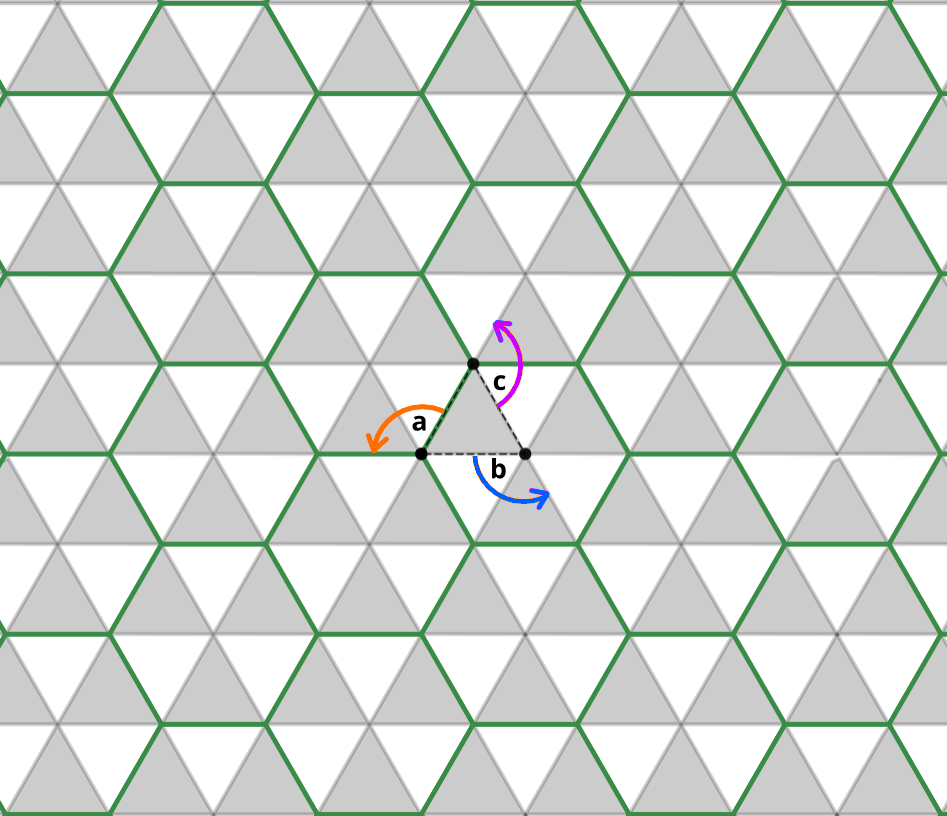
\includegraphics[height=60mm]{honey4}
 \caption{The realization of $\Delta_{(3,3,3)}$ as motions of the plane.} \label{fig:abc}
 \end{figure}

The elements $u=a^2b$, $v=aba$, $w=ba^2=u^{-1}v^{-1}$ correspond to the translations
of the pattern (see Figure~\ref{fig:abc}) by one step of length $\sqrt{3}$
in the directions north $\uparrow$,
southwest $\swarrow$ ($240^\circ$ north) and
southeast $\searrow$ ($120^\circ$ north), respectively.
They generate the abelian subgroup $\la u,v,w \ra \simeq \mbb{Z} \times \mbb{Z}$
of translations.
Note that the horizontal shift of length $1$ preserves the alternating triangles pattern,
but not the additional hexagonal. This is not an element of~$\Delta_{(3,3,3)}$.

One can see that
$\Delta_{(3,3,3)}/\la u,v,w \ra \simeq \mbb{Z}_3$.
Moreover,
\[
\Delta_{(3,3,3)} \simeq \mbb{Z}_3 \ltimes \la u,v,w \ra
\simeq \mbb{Z}_3 \ltimes (\mbb{Z} \times \mbb{Z}),
\]
where $\mbb{Z}_3$ acts by shifting the generators $u \rightarrow v \rightarrow w \rightarrow u$.
It follows from the identities $a^{-1}ua = v$, $a^{-1}va = w$ and $a^{-1}wa = u$.

We are interested in projective unitary representations of $\Delta_{(3,3,3)}$.
Denote the set of complex units by ${\rm S}^1 = \{\xi \in \mbb{C} \mid |\xi| = 1 \}$.

A \textit{projective unitary representation} of a group $G$
is a homomorphism from $G$ to the group
${\rm PUni}(n) = {\rm Uni}(n)/\la \xi I\ra$ of projective unitaries.
Alternatively, it is a map $\pi\colon G \longrightarrow {\rm Uni}(n)$ that satisfies
\begin{align*}
\pi(xy) = \pi(x)\pi(y) \cdot \xi(x, y),
\qquad
\xi(x, y) \in {\rm S}^1.
\end{align*}

Let $\pi$ be any such representation of $\Delta_{(3,3,3)}$.
It is easy to see that $(\pi(a))^3, (\pi(b))^3, (\pi(c))^3 \in \bigl\{ \gamma I \mid \gamma \in {\rm S}^1\bigr\}$.
Hence, we can choose scalars $\xi_a, \xi_b, \xi_c \in {\rm S}^1$ such that
\ea{\label{tri:ABC}
A^3 = B^3 = C^3 = I,\qquad ABC = \lambda I,
}
where $A = \xi_a\pi(a)$, $B = \xi_b\pi(b)$, $C = \xi_c\pi(c)$ and $\lambda \in {\rm S}^1$.
Henceforth, we focus on solving equation~\eqref{tri:ABC}.

Recall that two solutions $(A,B,C)$ and $(A',B',C')$
are unitary equivalent if and only if
\[
U(A,B,C)U^\dag = \bigl(UAU^\dag,UBU^\dag,UCU^\dag\bigr) = (A',B',C')
\]
for some $U \in {\rm Uni}(n)$.
A unitary representation $(A,B,C)$ is irreducible if and only if its not equivalent to
$(A',B',C') \oplus (A'',B'',C'') = (A'\oplus A'',B'\oplus B'',C'\oplus C'')$.
Equivalently, there is no proper subspace which is invariant for all $A$, $B$, $C$.

In fact, the irreducible unitary representations of equation~\eqref{tri:ABC} were
classified by Livinskyi and Radchenko in \cite{RL}. But here we present a modified and more
symmetric exposition of the results and also show the relation with Zauner's unitary.
Additionally, note that there is a~general (Mackey's) theory of finding representations
of virtually abelian groups~\cite{Kyr}.

By computing the determinants of expressions from equation~\eqref{tri:ABC}, one can conclude that $\lambda^{3n} = 1$,
so~$\lambda$ is a root of unity.
Denote $\mu = \lambda^3$ and let
\begin{align*}
U = A^2B,
\qquad
V = ABA,
\qquad
W = BA^2.
\end{align*}
%This definition will be used in the rest of the paper.
From equation~\eqref{tri:ABC}, it follows that
\ea{ \label{tri:UVW}
UV = \mu VU,
\qquad
VW = \mu WV,
\qquad
WU = \mu UW,
\qquad
UVW = \mu I,
\qquad
WVU = I.
}

The key idea is that we find irreducible representations of the equation \eqref{tri:UVW}
at first.
Then we find how $(U,V,W)$, that comes from an irreducible solution $(A,B,C)$,
can split into irreducible parts.
The representation theory of the relation $UV=\mu VU$ is well known \cite{Davidson,Weyl}.
If $\mu = \exp (2\pi k{\rm i}/d)  = \omega^k$, ${\rm gcd}(k,d)=1$,
then there are only $d$-dimensional irreducible representations which can be given by
\[
U_\alpha = \alpha Z^k,
\qquad
V_\beta = \beta X,
\]
where $\alpha, \beta \in {\rm S}^1$ are parameters of the representation.
Two such representations are equivalent if and only if
$\bigl(\alpha'^d, \beta'^d\bigr) = \bigl(\alpha^d, \beta^d\bigr)$. Thus the pair $\bigl(\alpha^d, \beta^d\bigr)$
specifies a representation uniquely.
Packed together, the irreducible $d$-dimensional solutions for $U$, $V$, $W$ in equation \eqref{tri:UVW}
can be described by
\begin{gather}
  U_\alpha = \alpha Z^k = \alpha D_{(0,k)},\qquad V_\beta = \beta X = \beta D_{(1,0)}, \qquad
 W_\gamma = \gamma \tau^k X^{-1}Z^{-k} = \gamma D_{(-1,-k)},\label{tri:UVWsol}
\end{gather}
where $\alpha \beta \gamma = \tau^k$.
And thus $\alpha^d \beta^d \gamma^d = \tau^{dk} = (-1)^{k(d-1)}$.

Two representations $(U_{\alpha'}, V_{\beta'}, W_{\gamma'})$ and $(U_\alpha, V_\beta, W_\gamma)$
are equivalent if and only if
\[
\bigl(\alpha'^d, \beta'^d, \gamma'^d\bigr) =\allowbreak \bigl(\alpha^d, \beta^d, \gamma^d\bigr).
\]

Let us return to the initial problem of finding irreducible solutions $(A,B,C)$ of equation~\eqref{tri:ABC}.
In general, the triple $(U,V,W) = \bigl(A^2B, ABA, BA^2\bigr)$, up to equivalence,
decomposes into a direct sum of irreducible summands given by equation~\eqref{tri:UVWsol}.
It corresponds to a decomposition of $H$ into invariant subspaces of $(U,V,W)$,
although this decomposition may not be unique if the summands are equivalent.
Let $H_1 \subseteq H$ be one of the invariant subspaces of dimension $d$.
Then the subspaces $H_2=A(H_1)$ and $H_3=A^2(H_1)$ are also invariant for $(U,V,W)$,
because $U(H_2) = \bigl(AVA^{-1}\bigr)(H_2) = AV(H_1) = A(H_1) = H_2$ and similarly for $H_3$ and $V, W$.
Since $H_1 + H_2 + H_3$ is invariant for $A$ as well as for $U$, $V$, $W$ we immediately obtain
that irreducible $(A,B,C)$ are at most~$3d$-dimensional.

Let us be more specific. Pick an orthonormal basis in $H_1$ so that
% \ea{\label{tri:H1}
\[
 (U,V,W)_{|_{H_1}} = (U_{\alpha},V_{\beta},W_{\gamma}),
\]
% }
for some parameters $(\alpha, \beta, \gamma)$ as in equation~\eqref{tri:UVWsol}.
This also fixes bases in $A(H_1)$ and $A^2(H_1)$ accordingly.
Then
% \ea{\label{tri:H2H3}
\begin{align*}
 & (U,V,W)_{|_{H_2}} = \bigl(A(V,W,U)A^{-1}\bigr)_{|_{A(H_1)}}
 = (V,W,U)_{|_{H_1}} = (V_{\beta},W_{\gamma},U_{\alpha}), \nn
 & (U,V,W)_{|_{H_3}} = \bigl(A^2(W,U,V)A^{-2}\bigr)_{|_{A^2(H_1)}}
 = (W,U,V)_{|_{H_1}} = (W_{\gamma},U_{\alpha}, V_{\beta}).
\end{align*}
% }

Consider the symplectic matrix
\[
M_{\mathfrak{Z}_k} = \bmp 0 & -k^{-1} \\ k & -1 \emp \in {\rm SL}(2, \mbb{Z}_{\bar{d}} )
\]
along with the symplectic unitary $\mathfrak{Z}_k \in {\rm Cli}(d)$ it generates
(we take a scalar such that $\mathfrak{Z}_k^3=1$).
$\mathfrak{Z}_k$ has order three and permutes $X \rightarrow Z^k \rightarrow D_{(-1,-k)} \rightarrow X$.
Hence,
\begin{align*}
 & \mathfrak{Z}_k(V_{\beta},W_{\gamma},U_{\alpha})\mathfrak{Z}_k^\dag
 = (U_{\beta},V_{\gamma},W_{\alpha}),
 \qquad \mathfrak{Z}_k^2(W_{\gamma},U_{\alpha},V_{\beta})\mathfrak{Z}_k^{2\dag}
 = (U_{\gamma},V_{\alpha},W_{\beta}).
\end{align*}

What we get is that the shift
$(U_{\alpha}, V_{\beta},W_{\gamma}) \rightarrow (V_{\beta},W_{\gamma},U_{\alpha})$
in a solution \eqref{tri:UVWsol} corresponds to
the change of parameters
$({\alpha}, {\beta}, {\gamma}) \rightarrow ({\beta}, {\gamma}, {\alpha})$.
Three shifts $(U_{\alpha}, V_{\beta},W_{\gamma})$, $(V_{\beta},W_{\gamma},U_{\alpha})$,
$(W_{\gamma},U_{\alpha},V_{\beta})$ are inequivalent unless
$\alpha^d = \beta^d = \gamma^d$, which can happen only in three cases
where \smash{$\alpha^d = \sqrt[3]{(-1)^{k(d-1)}}$} for three cubic root choices.
If shifts are inequivalent, then~$H_1$,~$H_2$,~$H_3$ should be orthogonal to each other
according to the representation theory.
In this case, the representation of $(A,B,C)$ is unique for
$\bigl({\alpha^d}, {\beta^d}, {\gamma^d}\bigr)$ and can be written as
\ea{\label{tri:abcsol}
A = \bmp
0 & 0 & I \\
I & 0 & 0 \\
0 & I & 0 \\
\emp,
\qquad
B = \bmp
0 & 0 & W_\gamma \\
U_\alpha & 0 & 0 \\
0 & V_\beta & 0 \\
\emp,
\qquad
C = \lambda\bmp
0 & 0 & U^\dag_{\alpha} \\
V^\dag_{\beta} & 0 & 0 \\
0 & W^\dag_{\gamma} & 0 \\
\emp,
}
in the chosen above basis in $H_1 \cup A(H_1) \cup A^2(H_1)$, with
\[
 U = \bmp
 U_\alpha & 0 & 0 \\
 0 & V_\beta & 0 \\
 0 & 0 & W_\gamma \\
 \emp,
 \quad
 V = \bmp
 V_\beta & 0 & 0 \\
 0 & W_\gamma & 0 \\
 0 & 0 & U_\alpha \\
 \emp,
 \quad
 W = \bmp
 W_\gamma & 0 & 0 \\
 0 & U_\alpha & 0 \\
 0 & 0 & V_\beta \\
 \emp.
\]

Let us consider the remaining situation
where \smash{$\alpha^d = \beta^d = \gamma^d = \sqrt[3]{(-1)^{k(d-1)}}$},
which we call \textit{the singularity case}.
We can assume that \smash{$\alpha = \beta = \gamma = \sqrt[3]{\tau^k}
= \omega_3^l \exp\bigl(\frac{\pi {\rm i} k(d+1)}{3d}\bigr)$}, $l=0,1,2$,
where $\omega_3 = \exp\bigl(\frac{2\pi{\rm i}}{3}\bigr)$. Define
\begin{align*}
& H_1' = \bigl\{\ket{f} + A^{-1}\mathfrak{Z}_k\ket{f} + A^{-2}\mathfrak{Z}_k^{2}\ket{f} \mid  \ket{f} \in H_1 \bigr\} \subset H, \\
 &H_2' = \bigl\{\ket{f} + \omega_3A^{-1}\mathfrak{Z}_k\ket{f} + \omega_3^2A^{-2}\mathfrak{Z}_k^{2}\ket{f} \mid  \ket{f} \in H_1 \bigr\} \subset H, \\
& H_3' = \bigl\{\ket{f} + \omega_3^2A^{-1}\mathfrak{Z}_k\ket{f} + \omega_3A^{-2}\mathfrak{Z}_k^{2}\ket{f} \mid  \ket{f} \in H_1 \bigr\} \subset H.
\end{align*}
One can see that $H_1'$ is invariant for $A$
and
\begin{align*}
 U(\ket{f} + A^{-1}\mathfrak{Z}_k\ket{f} + A^{-2}\mathfrak{Z}_k^{2}\ket{f})
 &= U \ket{f} + A^{-1}W\mathfrak{Z}_k\ket{f} + A^{-2}V\mathfrak{Z}_k^{2}\ket{f} \\
 &= U_\alpha \ket{f} + A^{-1}W_\alpha\mathfrak{Z}_k\ket{f} + A^{-2}V_\alpha\mathfrak{Z}_k^{2}\ket{f}\\
& = U_\alpha \ket{f} + A^{-1}\mathfrak{Z}_kU_\alpha\ket{f} + A^{-2}\mathfrak{Z}_k^{2}U_\alpha\ket{f}
 \in H_1',
\end{align*}
so it is invariant for $U$ and thus for $V$ and $W$ too. The same holds
for $H_2'$, $H_3'$. Note that $H_1'+H_2'+H_3' = H_1+H_2+H_3$ and $\dim H_i'$ is
either $d$ or $0$ for each $i$ due to invariance.
Hence, $\dim H_i' = d$ for at least one index $i$.
But this means that irreducible representations of $(A,B,C)$
are at most $d$-dimensional in this case and we should have $H_1=H_2=H_3$
from the beginning.
It follows that~$A$ is an automorphism of $\la U, V, W\ra = \la U_\alpha, V_\alpha, W_\alpha\ra$
since $V = A^{-1}UA$, $W = A^{-2}UA^2$.
From the description of ${\rm Cli}(d)$, we know that $A$ coincides with $\mathfrak{Z}_k$ up to $\omega_3$ factor.
We conclude that there are three inequivalent representations
\begin{gather}
 A = \omega_3^j \mathfrak{Z}_k,
 \qquad B = \omega_3^j \mathfrak{Z}_k U_\alpha,
\qquad C = \lambda \omega_3^j U_\alpha^\dag \mathfrak{Z}_k,\nonumber \\
 U = U_\alpha,
\qquad V = V_\alpha,
\qquad W = W_\alpha,\label{tri:aaasol}
\end{gather}
where $j=0,1,2$ for each \smash{$\alpha = \sqrt[3]{\tau^k}$}, so that is 9 in total.
Moreover, the representation \eqref{tri:abcsol} decomposes exactly into
the three parts that correspond to the values of $j=0,1,2$ each, where the invariant subspaces are
$H'_{j+1}$.
We summarize this in the following theorem, which refines \cite[Theorem~5]{RL}:
\begin{Theorem}\label{tri:thm}
Let $\mu = \lambda^3 = \exp (2\pi k {\rm i}/d) = \omega^k$, ${\rm gcd}(k,d)=1$.
Consider the set of parameters~${(\alpha, \beta, \gamma) \in {\rm S}^1 \times {\rm S}^1 \times {\rm S}^1}$
with $\alpha\beta\gamma = \tau^k$ and
the equivalence relation $\bigl(\alpha'^d, \beta'^d, \gamma'^d\bigr) = \bigl(\alpha^d, \beta^d, \gamma^d\bigr)$.
Then equations \eqref{tri:abcsol}
define inequivalent irreducible $3d$-dimensional representations of \eqref{tri:ABC},
except three cases where \smash{$\alpha^d = \beta^d = \gamma^d = \sqrt[3]{(-1)^{k(d-1)}}
= \omega_3^l (-1)^{k(d-1)}$}, $l=0,1,2$.
In each of those cases, equations~\eqref{tri:abcsol} split into three inequivalent irreducible
$d$-dimensional representations \eqref{tri:aaasol}, generating nine in total.
\end{Theorem}

In the simplest case, $\lambda^3 = 1$ and $d=k=1$, $\omega=\tau=1$. For three complex units with
$\alpha\beta\gamma=1$, we have $U_\alpha = \alpha$, $U_\beta = \beta$, $U_\gamma = \gamma$ and
equation~\eqref{tri:abcsol} reads as
\[
A = \bmp
0 & 0 & 1 \\
1 & 0 & 0 \\
0 & 1 & 0 \\
\emp,
\qquad
B = \bmp
0 & 0 & \gamma \\
\alpha & 0 & 0 \\
0 & \beta & 0 \\
\emp,
\qquad
C = \lambda\bmp
0 & 0 & \bar{\alpha} \\
\bar{\beta} & 0 & 0 \\
0 & \bar{\gamma} & 0 \\
\emp.
\]

This solution will be reducible if $\alpha=\beta=\gamma=\omega_3^l$.
Since $\mathfrak{Z}_k=1$ (up to $\omega_3$ factor), equations~\eqref{tri:aaasol} give the irreducible parts where $j=0,1,2$,
\[
 A = \omega_3^j,
\qquad B = \omega_3^{j+l},
\qquad C = \lambda \omega_3^{j-l}.
\]

We remark that in general $U_\alpha^d = \alpha^d I$ and similarly for $\beta$, $\gamma$.
This helps to understand how, in a general representation, the tuple $(U,V,W)$ decomposes into
irreducible parts. We will look at the spectral decompositions of $U^d$, $V^d$ and $W^d$.

\begin{thebibliography}{99}
\bibitem[2]{Appleby}
Appleby D.M., Symmetric informationally complete-positive operator valued
 measures and the extended {C}lifford group, \href{https://doi.org/10.1063/1.1896384}{\textit{J.~Math. Phys.}}
 \textbf{46} (2005), 052107, 29~pages, \href{https://arxiv.org/abs/quant-ph/0412001}{arXiv:quant-ph/0412001}.

\bibitem[8]{BosWal}
Bos L., Waldron S., S{IC}s and the elements of order three in the {C}lifford
 group, \href{https://doi.org/10.1088/1751-8121/aafff3}{\textit{J.~Phys.~A}} \textbf{52} (2019), 105301, 31~pages.

\bibitem[9]{Davidson}
Davidson K.R., {$C^*$}-algebras by example, \textit{Fields Inst. Monogr.},
 Vol.~6, \href{https://doi.org/10.1090/fim/006}{American Mathematical Society}, Providence, RI, 1996.

\bibitem[10]{Fla}
Flammia S.T., On {SIC}-{POVM}s in prime dimensions, \href{https://doi.org/10.1088/0305-4470/39/43/007}{\textit{J.~Phys.~A}}
 \textbf{39} (2006), 13483--13493, \href{https://arxiv.org/abs/quant-ph/0605050}{arXiv:quant-ph/0605050}.

\bibitem[12]{Kyr}
Kirillov A.A., Elements of the theory of representations, \textit{Grundlehren
 Math. Wiss.}, Vol. 220, \href{https://doi.org/10.1007/978-3-642-66243-0}{Springer}, Berlin, 1976.

\bibitem[14]{RL}
Livins'kyi I.V., Radchenko D.V., Representations of algebras defined by a
 multiplicative relation and corresponding to the extended {D}ynkin graphs
 {$\tilde{D}_4$}, {$\tilde{E}_6$}, {$\tilde{E}_7$}, and {$\tilde{E}_8$},
 \href{https://doi.org/10.1007/s11253-013-0757-y}{\textit{Ukrainian Math.~J.}} \textbf{64} (2013), 1865--1892.

\bibitem[15]{Magnus}
Magnus W., Noneuclidean tesselations and their groups, \textit{Pure Appl.
 Math.}, Vol.~61, Academic Press, New York, 1974.

\bibitem[17]{Scott2}
Scott A.J., {SIC}s: {E}xtending the list of solutions, \href{https://arxiv.org/abs/1703.03993}{arXiv:1703.03993}.

\bibitem[19]{SG}
Scott A.J., Grassl M., Symmetric informationally complete
 positive-operator-valued measures: a new computer study, \href{https://doi.org/10.1063/1.3374022}{\textit{J.~Math.
 Phys.}} \textbf{51} (2010), 042203, 16~pages, \href{https://arxiv.org/abs/0910.5784}{arXiv:0910.5784}.

\bibitem[20]{Weyl}
Weyl H., The theory of groups and quantum mechanics, Dover Publications, New
 York, 1950.

\end{thebibliography}
\end{document}
